\subsubsection{UC15.1 - Inserimento valore da modificare}
\begin{figure}[H]
	\centering
	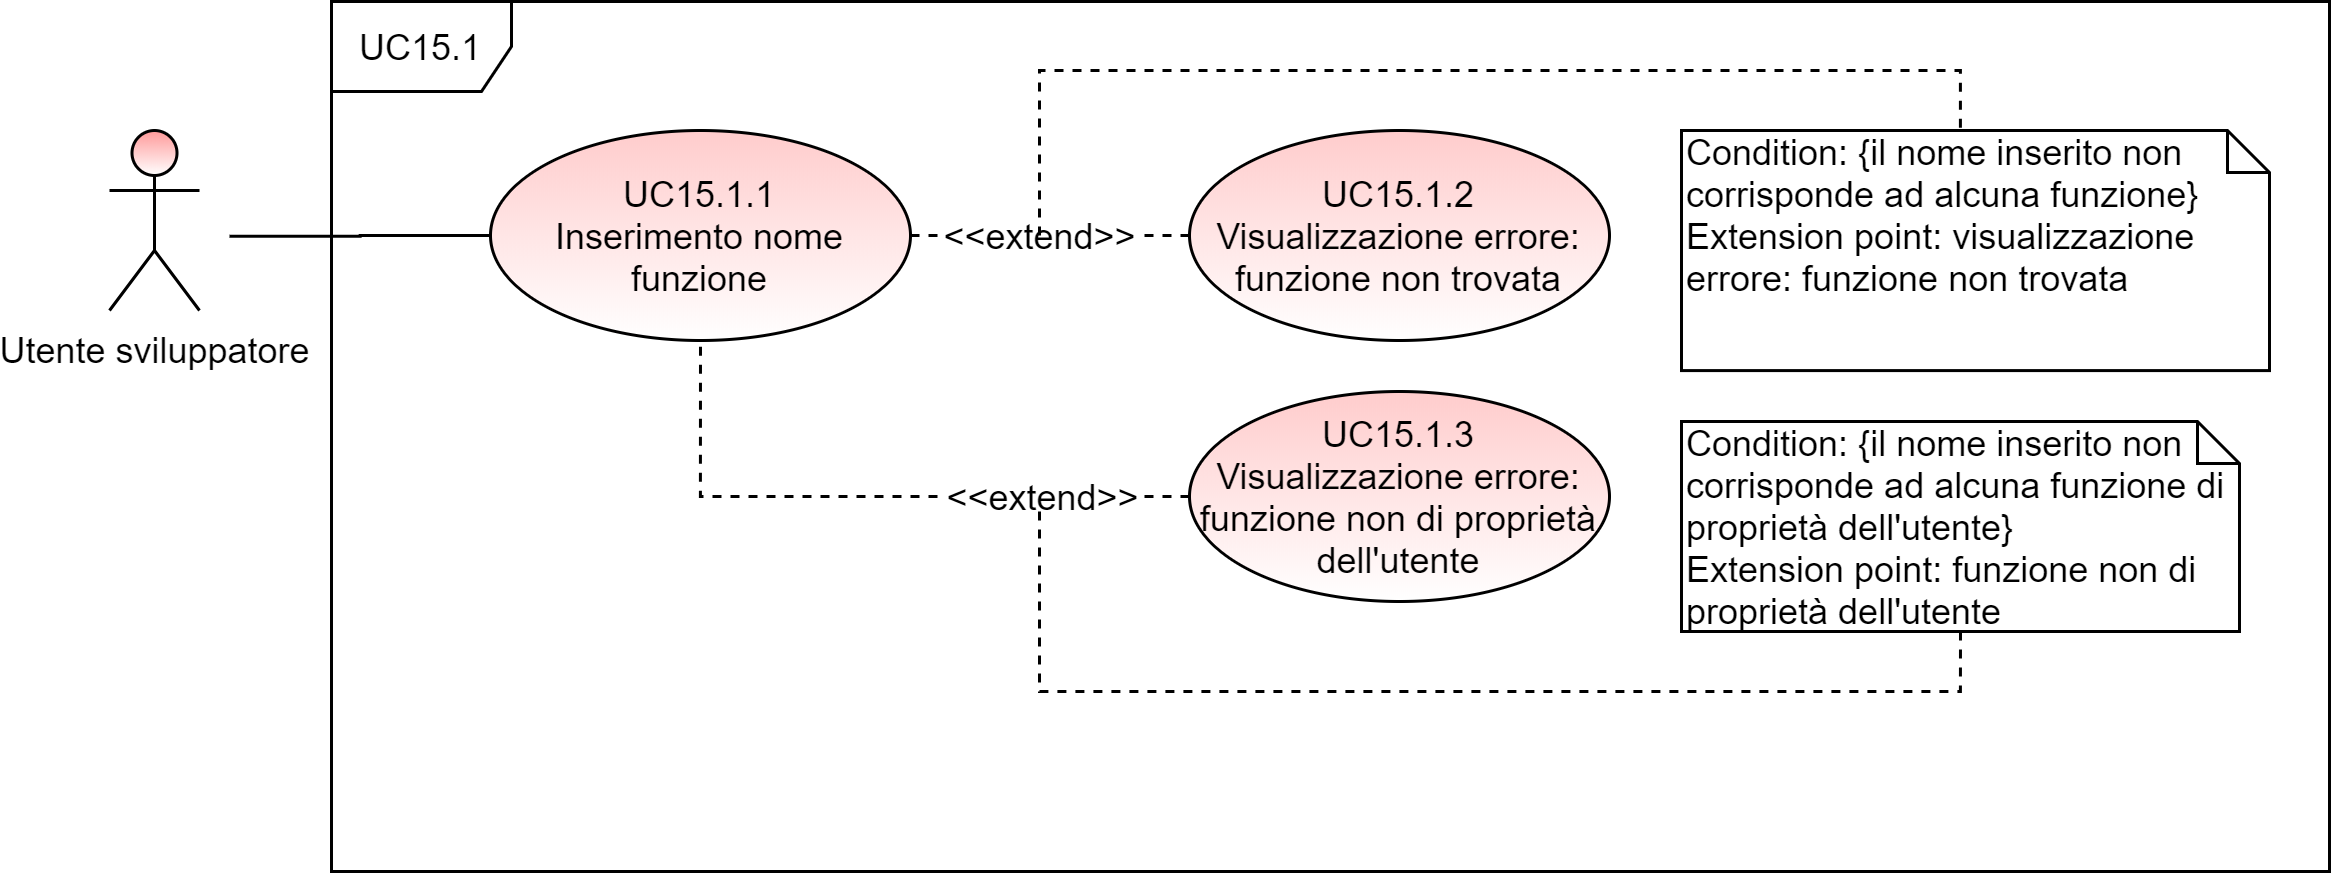
\includegraphics[scale=\ucs]{./res/img/UC15-1.png}
	\caption {UC15.1 - Inserimento valore da modificare}
\end{figure}
\begin{itemize}
	\item \textbf{Attori primari:} \us{};
	\item \textbf{Descrizione:} a seguito dell'inserimento del comando \edit{} l’utente procede con l’inserimento del nome della funzione considerata e delle modifiche da apportare; 
	\item \textbf{Scenario principale:} l'utente inserisce il comando \edit{} seguito dal nome della funzione e dalle infrormazioni da aggiornare; 
	\item \textbf{Specializzazioni:} 
	\begin{itemize}
		\item \textbf{UC15.2:} l’utente vuole modificare la descrizione della funzione considerata; 
		\item \textbf{UC15.3:} l’utente vuole modificare il codice della funzione. 
	\end{itemize}
	\item \textbf{Precondizione:} l’utente ha inserito all’interno della CLI\ped{\textit{G}} il comando \edit{}; 
	\item \textbf{Postcondizione:} l’utente ha inserito correttamente le nuove informazioni relative alla funzione.
\end{itemize}